\clearpage

\lehead[]{\sf\hspace*{-2.00cm}\textcolor{white}{\colorbox{lightblue}{\makebox[1.60cm][r]{\thechapter}}}\hspace{0.17cm}\textcolor{lightblue}{\chaptertitle}}
\rohead[]{\textcolor{lightblue}{\chaptertitle}\sf\hspace*{0.17cm}\textcolor{white}{\colorbox{lightblue}{\makebox[1.60cm][l]{\thechapter}}}\hspace{-2.00cm}}
%\chead[]{}
\rehead[]{\textcolor{lightblue}{AvHG, Inf, My}}
\lohead[]{\textcolor{lightblue}{AvHG, Inf, My}}

\lstset{style=myJava}


\section{Eine mögliche Lösung: Brute Force}

Es gibt viele mögliche Algorithmen, um die Quadratwurzel einer beliebigen
positiven Zahl zu bestimmen.

Ein ganz einfacher Ansatz basiert auf dem Wissen, dass die Lösung irgendwo im
Bereich von 0,0 und Unendlich liegen muss. Folglich könnte man bei Null
beginnend und mit einer hinreichend kleinen Schrittweite alle mögliche Lösungen
durchprobieren (je kleiner wir die Schrittweite wählen, desto genauer wird
unser Ergebnis sein).

Das Programm als sogenannter \emph{Pseudocode}:

\begin{lstlisting}
radikand = benutzereingabe()
gerateneLösung = 0.0
quadrat = gerateneLösung * gerateneLösung
schrittweite = 0.0001

WIEDERHOLE SOLANGE (quadrat < radikand):
    gerateneLösung = gerateneLösung + schrittweite
    quadrat = gerateneLösung * gerateneLösung

PRINT gerateneLösung
\end{lstlisting}

Der gleiche Algorithmus als sogenanntes \emph{Flussdiagramm} (englischer
Fachausdruck \emph{Flowchart}):

\begin{figure}[h]
  \centering
   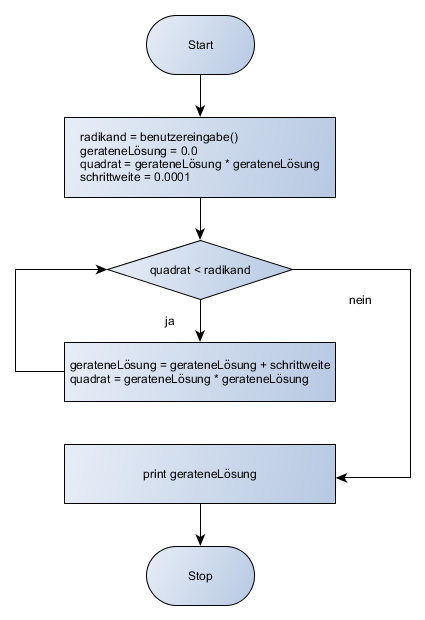
\includegraphics[width=0.6\textwidth]{./inf/SEKII/03_Informatik/Flussdiagramm_Wurzel_Brute-Force.png}
   \caption{Flussdiagramm: Ermittlung der Quadratwurzel mit dem
   Brute-Force-Verfahren}
   \label{fig:flussdiagramm-wurzel-brute-force}
\end{figure}

Dieser Algorithmus ist gut in dem Sinne, dass der Lösungsweg direkt einleuchtend
ist. Außerdem ist er sehr kurz.

Alles andere als kurz (und gut) ist allerdings der nötige Aufwand, der so zu
betreiben ist: Selbst um die Quadratwurzel von 100 zu bestimmen, sind bei
der oben gewählten Schrittweite bereits 100000 (einhunderttausend)
Wiederholungen der Schleife nötig, um das Ergebnis zu finden.


\section{Eine bessere mögliche Lösung: Bisektion}

Statt -- wie im ersten Lösungsansatz -- stumpf alle Möglichkeiten
durchzuprobieren (solch eine Lösungsstrategie wird oft als \emph{Exhaustive
Enumeration} oder auch \emph{Brute Force} bezeichnet), gibt es oft
intelligentere Ansätze, durch die der Rechenaufwand erheblich reduziert werden
kann.

\emph{Bisektion} ist solch ein Ansatz. Er wird oft verwendet, wenn eine Lösung
in einer großen, aber geordneten Lösungsmenge gesucht wird. Ein Zahlenstrahl --
etwa die Menge der Reellen Zahlen -- ist solch eine geordnete Lösungsmenge.
Geordnet in dem Sinne, dass alle Zahlen links von einer gegebenen Zahl kleiner
sind als diese und alle Zahlen rechts von ihr größer.

Wenn wir zu Beginn eine Ober- und eine Untergrenze für die mögliche Lösung
kennen, dann wissen wir in welchem Bereich der Lösungsmenge wir nach unserer
richtigen Lösung suchen müssen. Suchen wir etwa die Quadratwurzel eine positiven
Zahl, die größer als 1 ist, so wissen wir, dass die Lösung irgendwo im
Bereich zwischen 0 und der gewählten positive Zahl (dem Radikand) liegen muss.

Das Bisektions-Verfahren teilt nun einfach immer wieder die Lösungsmenge in zwei
gleich große Teile und testet, ob sich die Lösung in der oberen oder unteren
Hälfte befindet. Und wiederholt diese Teilung (mit den jeweils neu gefundenen
Ober- und Untergrenzen) solange, bis die Lösung hinreichend genau bestimmt
wurde.

In unserem Beispiel aus dem Brute-Force-Ansatz (oben), wurde die Quadratwurzel
von 100 gesucht.

Mit dem Bisektionsansatz würden wir zu Beginn als untere Grenze unserer
Lösungsmenge 0 und als obere Grenze 100 setzen. Diese Lösungsmenge teilen wir
nun in zwei gleich große Hälften und müssen entscheiden, in welcher der beiden
Hälften die richtige Lösung liegt. Um dies zu entscheiden prüfen wir, ob

$$
\left(\frac{\textrm{untere Grenze} \,+\, \textrm{obere Grenze}}{2}\right)^2 \; =
\; \left(\frac{0 \,+\, 100}{2}\right)^2 ~=~ 50^2 ~=~ 2500
$$

größer oder kleiner als unser Radikand (100) ist. Der Ausdruck ist größer. Also
wissen, dass wir in der unteren Hälfte der ursprünglichen Lösungsmenge nach der
richtigen Lösung suchen müssen und die obere Hälfte komplett ignorieren können.
Wir haben also in einem Schritt die Lösungsmenge halbiert!

Die neue obere Grenze ist nun 50. Die untere Grenze ist unverändert geblieben.

Wieder teilen wir unsere Lösungsmenge in zwei gleich große Teile. Und wieder
überprüfen wir, ob

$$
\left(\frac{\textrm{untere Grenze} \,+\, \textrm{obere Grenze}}{2}\right)^2 \; =
\; \left(\frac{0 + 50}{2}\right)^2 ~=~ 25^2 ~=~ 625
$$

größer oder kleiner als der gegebene Radikand ist.

Und so weiter, und so weiter. Bereits nach 22 Schritten, haben wir die Lösung
auf mindestens vier Nachkommastellen genau bestimmt! Noch mal zum Vergleich: Mit
der Brute-Force-Methode waren es einhunderttausend Schritte!

\pagebreak

Hier das passende Programm als Pseudocode:

\begin{lstlisting}
radikand = benutzereingabe()
akzeptierterFehler = 0.0001
untereGrenze = 0.0
obereGrenze = MAXIMUM(1, radikand)
gerateneLösung = (untereGrenze + obereGrenze) / 2
quadrat = gerateneLösung * gerateneLösung
abweichung = BETRAG(quadrat - radikand)

WIEDERHOLE SOLANGE (abweichung > akzeptierterFehler):
    FALLS (quadrat > radikand):
        obereGrenze = gerateneLösung
    SONST:
        untereGrenze = gerateneLösung
    gerateneLösung = (untereGrenze + obereGrenze) / 2
    quadrat = gerateneLösung * gerateneLösung
    abweichung = BETRAG(quadrat - radikand)

PRINT gerateneLösung
\end{lstlisting}

Wer genau hinschaut sieht, dass dieses Programm noch den Fall berücksichtigt,
dass der Radikand kleiner als 1 ist. Dann liegt die gesuchte Lösung nicht im
Bereich zwischen 0 und dem gegebenen Radikand, sondern zwischen 0 und 1!

Abbildung \ref{fig:flussdiagramm-wurzel-bisektion} (nächste Seite) zeigt das
passende Flussdiagramm.

\begin{figure}[h]
  \centering
   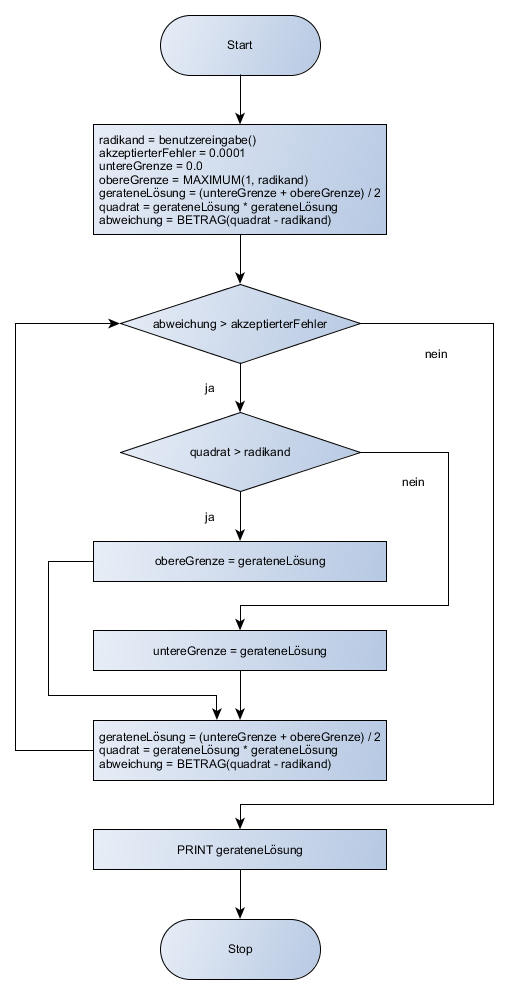
\includegraphics[width=0.7\textwidth]{./inf/SEKII/03_Informatik/Flussdiagramm_Wurzel_Bisektion.png}
   \caption{Flussdiagramm: Ermittlung der Quadratwurzel mit dem
   Bisektionsverfahren}
   \label{fig:flussdiagramm-wurzel-bisektion}
\end{figure}

\clearpage

\section{Implementierung in echten Programmiersprachen}

Auf der nächsten Doppelseite seht ihr, wie der bisher in Pseudocode und als
Flussdiagramm  beschriebene Algorithmus tatsächlich -- also mit einer \glqq
echten\grqq\ Programmiersprache -- implementiert werden kann.

Es gibt viele verschiedene Programmiersprachen. Und natürlich gibt es
Unterschiede zwischen ihnen. Die Kontrollstrukturen, wie bedingte Anweisungen,
Verzweigungen und Schleifen, haben aber die allermeisten Programmiersprachen
gemein.

Beispielhaft wurde hier die Implementierung einmal in Python und einmal in Java
gewählt. Bei beiden handelt es sich um imperative, objektorientierte
Programmiersprachen. Im Unterschied zu Java muss man in Python aber den Datentyp
von Variablen nicht vorab bestimmen (Java gehört zu den \emph{stark
typisierenden} Sprachen, Python nicht).

Außerdem unterscheiden sich verschiedene Programmiersprachen durch die
vorgefertigten Funktionen, etwa zur Ein- und Ausgabe von Text, oder auch für
mathematische Funktionen wie zur Bestimmung des Maximums mehrerer
gegebener Werte oder auch des Betrages einer Zahl.

Manche Programmiersprachen sind für spezielle Aufgabenzwecke konzipiert (etwa
die Programmiersprache R, die oft für statistische Auswertungen benutzt wird),
andere sind sogenannte \emph{General Purpose} Programmiersprachen. Sowohl Java
als auch Python gehören zu diesem allgemeinen Typ.

Welche Programmiersprache man bevorzugt bzw. einsetzt hängt zum einem von
persönlichen Vorlieben ab, zum anderen von möglichen Vorgaben. So wie etwa bei
uns im Informatik-Unterricht: Wir werden im weiteren Verlauf mit Java arbeiten. 

\clearpage

\subsection{Implementierung in Python}

\begin{lstlisting}
radikand = float(raw_input('Gib eine positive Zahl ein: '))
akzeptierterFehler = 0.0001
æanzahlSchritte = 0æ
untereGrenze = 0.0
obereGrenze = max(1.0, radikand)
gerateneLoesung = (untereGrenze + obereGrenze) / 2.0
quadrat = gerateneLoesung * gerateneLoesung
abweichung = abs(quadrat - radikand)

while abweichung > akzeptierterFehler:
    æanzahlSchritte += 1æ
    if quadrat < radikand:
        untereGrenze = gerateneLoesung
    else:
        obereGrenze = gerateneLoesung
    gerateneLoesung = (obereGrenze + untereGrenze) / 2.0
    quadrat = gerateneLoesung * gerateneLoesung
    abweichung = abs(quadrat - radikand)

æprint 'Anzahl Schritte =', anzahlSchritteæ
print gerateneLoesung, 'ist die Quadratwurzel von', radikand
\end{lstlisting}

\clearpage

\subsection{Implementierung in Java}

\begin{lstlisting}
import java.util.Scanner;

public class Qudratwurzel {

	public static void main(String[] args) {
		double radikand;
		double akzeptierterFehler = 0.0001;
		æint anzahlSchritte = 0;æ
		double untereGrenze = 0.0;
		double obereGrenze;
		double gerateneLösung;
		double quadrat;
		double abweichung;

		Scanner scanner = new Scanner(System.in);
		System.out.print("Gib eine positive Zahl ein: ");
		radikand = scanner.nextDouble();               æ// Eingabe mit Komma statt Punkt! 
æ	    obereGrenze = Math.max(1.0, radikand);
		gerateneLösung = (untereGrenze + obereGrenze) / 2.0;
		quadrat = gerateneLösung * gerateneLösung;
		abweichung = Math.abs(quadrat - radikand);

		while (abweichung > akzeptierterFehler) {
			æanzahlSchritte++;æ
			if (quadrat < radikand) {                    æ// Die geratene Wurzel ist zu klein
æ			    untereGrenze = gerateneLösung;
			} else {                                     æ// Die geratene Wurzel ist zu groß
æ			    obereGrenze = gerateneLösung;
			}
			gerateneLösung = (obereGrenze + untereGrenze) / 2.0;
			quadrat = gerateneLösung * gerateneLösung;
			abweichung = Math.abs(quadrat - radikand);
		}

		æSystem.out.println("Anzahl Schritte = " + anzahlSchritte);æ
		System.out.println(gerateneLösung + " ist die Quadratwurzel von " + radikand);
	}

}
\end{lstlisting}


\clearpage

\section{Wer es genauer wissen will}

\url{http://de.wikipedia.org/wiki/Pseudocode}

\url{http://de.wikipedia.org/wiki/Programmablaufplan} (Flussdiagramme)

\url{http://de.wikipedia.org/wiki/Brute-Force-Methode}

\url{http://de.wikipedia.org/wiki/Bisektion}

\url{http://de.wikipedia.org/wiki/Programmiersprache}


